\documentclass{standalone}
\usepackage[margin=1in]{geometry}
\usepackage[hang,small,bf]{caption}
\usepackage{tikz}
\usepackage{braket}
\usetikzlibrary{backgrounds,shadows.blur,fit,decorations.pathreplacing,shapes}
\begin{document}
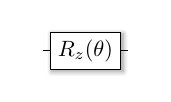
\begin{tikzpicture}[scale=0.8, transform shape]
\tikzstyle{basicshadow}=[blur shadow={shadow blur steps=8, shadow xshift=0.7pt, shadow yshift=-0.7pt, shadow scale=1.02}]
\tikzstyle{basic}=[draw,fill=white, basicshadow]
\tikzstyle{operator}=[basic, minimum size=1.5em]
\tikzstyle{phase}=[fill=black, shape=circle, minimum size=5pt, inner sep=0pt, outer sep=-1pt,basicshadow]
\tikzstyle{none}=[inner sep=0pt, outer sep=-.5pt, minimum height=0.5cm+1pt]
\tikzstyle{measure}=[basic, inner sep=0.5em, minimum height=1.7em, minimum width=2.5em]
\tikzstyle{xstyle}=[circle, basic, minimum height=.25cm, minimum width=.25cm]
\tikzset{ 
shadowed/.style={preaction={transform canvas={shift={(0.5pt,-0.5pt)}}, draw=gray, opacity=0.4}},
}
\tikzstyle{swapstyle}=[shadowed, inner sep=0pt, outer sep=0pt, minimum width=0pt]
\tikzstyle{edgestyle}=[thin]
\node at (1,.25) {};
\node at (0.5,-0) (op0o0) {};
%\node[xstyle] (op0o1) at (1,-0) {};
%\draw[edgestyle] (op0o1.north)--(op0o1.south);
%\draw[edgestyle] (op0o1.west)--(op0o1.east);

\node[operator] (op0o1) at (1.3,0) {$R_z(\theta)$};
\draw (op0o0) edge[edgestyle]  (op0o1);
\node (op0o2) at (2.1,-0) {};
\draw (op0o1) edge[edgestyle]  (op0o2);
\node at (1,-.25){};
\end{tikzpicture}
\end{document}
